\documentclass[10pt,a4paper]{article}
\usepackage[margin=1.35cm]{geometry}
\usepackage{graphicx,amsmath,booktabs,siunitx}
\usepackage[font=small,labelfont=bf]{caption}
\usepackage[hidelinks]{hyperref}
\graphicspath{{../output/}}
\setlength{\parskip}{0.4em}\setlength{\parindent}{0pt}

\title{Do mesoscope neurons keep their task responses across days?}
\author{Chronic-stability pilot (\texttt{pilot\_analyses/chronic\_stability})}
\date{\today}

\begin{document}
\maketitle

\section{Methods}

\paragraph{Data.}
We used the six mice whose mesoscope sessions have ROICaT cross-session neuron identities on the FlatIron mirror
(SP054, SP058, SP061, SP066, SP067, SP072): 83 sessions in total (3--23 per mouse, each mouse spanning 6--52 days;
82--742 trials per session, median 5\,100--8\,500 neurons per session; Table~\ref{tab:data}).
Mice performed the IBL visual decision task. For every session we took the per-trial deconvolved activity
already extracted for the dorsal-maps analysis, averaged in 9 windows: stimulus onset 0--0.3\,s, pre-movement
$-0.3$--0\,s, feedback 0--0.3\,s, and six 0.2\,s bins from $-0.2$ to 1.0\,s around first movement.
We kept ROIs classified as neurons, located in isocortex, and with valid atlas coordinates.

\begin{table}[h]
\centering\small
\begin{tabular}{lrrrrrrr}
\toprule
mouse & sessions & days & neurons/session & tracked in $\geq$half & $\geq$80\% & all sessions & session pairs\\
\midrule
SP054 & 10 & 18 & 5\,117 & 1\,517 & 312 & 28 & 36\\
SP058 & 23 & 44 & 8\,441 & 4\,905 & 468 & 67 & 253\\
SP061 & 10 & 52 & 8\,502 & 6\,147 & 1\,998 & 329 & 45\\
SP066 & 3 & 6 & 7\,129 & 5\,585 & 2\,256 & 2\,256 & 3\\
SP067 & 20 & 29 & 8\,168 & 4\,239 & 254 & 0 & 154\\
SP072 & 18 & 36 & 8\,365 & 5\,224 & 895 & 211 & 153\\
\bottomrule
\end{tabular}
\caption{Dataset. Tracked counts include only QC-passing matches. \emph{Session pairs}: the number of pairs of sessions of the same mouse that met all criteria for the across-day comparison. Of $n$ usable sessions at most $n(n-1)/2$ pairs are possible. Criteria: (i) each session has $\geq$5 trials of each trial type (rewarded left, rewarded right, unrewarded) in both the even and the odd half; (ii) the two sessions share $\geq$50 tracked neurons that pass the tracking QC in both. All possible pairs met the criteria except in SP054, where one of the 10 sessions (2024-02-07, a single trial) failed (i) (9 sessions, 36 pairs), and SP067, where 154 of 190 pairs met (ii); its last two sessions come from a separate ROICaT run and share no IDs with the rest. Pairs share sessions and are therefore not independent; statistics are computed per mouse.}
\label{tab:data}
\end{table}

\paragraph{Tracking.}
Neuron identities across sessions come from an existing ROICaT run; we did not run the tracking ourselves.
For each session and FOV we downloaded \texttt{alf/FOV\_XX/mpciROIs.clusterUIDs.csv} from the FlatIron mirror
(\url{https://ibl.flatironinstitute.org/resources/mesoscope/ROICaT/<subject>/<date>/<number>/}).
Each file has one line per ROI, in ROI order; the same ID string in two sessions marks the same cell, and an empty line means the ROI is untracked.
FOV numbers can change between sessions (e.g.\ SP058 FOV\_04 becomes FOV\_05 from 2024-07-29), and ROICaT follows neurons across such renumbering.
IDs were assigned to the feature rows by rebuilding the row selection from the ROI files, checking that the row count and the atlas IDs agree.
This check failed for SP058 after a histology update had changed the selection, so its 23 sessions were re-extracted.
The mirror gives only the IDs, not ROICaT's match-quality scores, so we checked each match from ROI positions (\texttt{mpciROIs.stackPos}).
Every pair of (session, FOV) sharing $\geq$20 IDs was registered with a robust affine transform fitted on the shared neurons' pixel positions, refitting after removing outliers more than 3 MAD away.
A neuron's deviation in a session is the median of its registration residuals over all pairs that include it.
A match passes when this deviation is smaller than half the distance to the nearest other neuron ROI in that FOV, so it cannot be a swap with that neighbour.
95.3\% of (neuron, session) entries pass: median deviation 1.5\,px (about 3\,\textmu m) against a median nearest-neighbour distance of 8.3\,px.
Only passing entries are used below.

\paragraph{Baseline: even vs.\ odd trials.}
Every metric is computed on half the trials.
Within a session, the metric compares even with odd trials, which gives the noise ceiling.
Across days $a$ and $b$, it compares even trials of $a$ with odd trials of $b$ (and odd $a$ with even $b$, averaged), so both comparisons use the same amount of data.
Each across-day value is expressed as the fraction of its within-session baseline kept: 1 means as reproducible as within a session, 0 means chance.

\paragraph{Metrics} (computed per session pair, on neurons tracked in both sessions):
\begin{itemize}\itemsep0pt
\item \emph{Response profile}: trial-mean activity in the 9 windows for rewarded-left, rewarded-right and unrewarded trials (27 values; errors pooled over sides).
Per neuron we computed the profile correlation within a day ($r_w$), across days ($r_x$), with a random neuron of the same FOV across days ($r_0$), and with the spatially nearest tracked neuron across days ($r_{nn}$).
Stability index $=(\tilde r_x-\tilde r_0)/(\tilde r_w-\tilde r_0)$ on medians.
\item \emph{Activity level}: correlation across neurons of log mean activity.
\item \emph{Selectivity maps}: correlation across neurons of $d'$ for stimulus side (contra vs.\ ipsi to the recorded hemisphere, stimulus window), choice (pre-movement window) and reward (feedback window).
\item \emph{Sensitivity persistence}: among neurons significantly stimulus- or choice-selective on one half (Mann--Whitney $p<0.01$), the fraction also significant with the same sign on the other half. Chance is half the fraction of significant neurons.
\item \emph{Population decoder}: ridge classifier (dual form, GPU; validated against \texttt{sklearn}) for stimulus side and choice from all tracked neurons. Trained on even trials of day $a$, tested on odd trials of day $a$ or day $b$; balanced accuracy. Chance was estimated by retraining the across-day decoders on 50 random permutations of the training labels (mean 0.500 for both variables; 95th percentile of a single pair $\approx$0.56--0.57).
\end{itemize}
Session pairs were grouped by days apart (1--2, 3--7, 8--14, 15--30, $>$30), averaged per mouse, then across mice.
For the decline with time, we fitted a slope of each normalised metric against $\log_{10}$(days apart) per mouse and tested it with a $t$-test across mice.
SP066 has only 6 days and was excluded from this test.
\emph{Single-neuron trends}: for neurons tracked in $\geq$6 sessions and stimulus-selective overall (mean sign-aligned $d'>0.2$), we computed the slope of $d'$ against recording day.
This slope was compared with 2\,000 shuffles of the session order; a neuron counts as losing or gaining selectivity at $p<0.025$ per tail.

\paragraph{Regions.}
The profile stability index was also computed separately per cortical region (\texttt{regions.py}). We chose it because it is the most robust metric: every tracked neuron counts, there is no significance threshold, it is scale-free, and it is normalised by both chance and the within-day baseline, so it compares fairly between regions with different reliability or neuron numbers.
Each neuron was assigned the Beryl region of its ROI centre in the Allen CCF; it counted for a region only if both sessions of the pair placed it there. AUDp, AUDpo and AUDd were pooled (AUD). Six regions had enough data: VISp, VISal, VISrl, VISa, SSp-bfd and AUD. A region entered a session pair only with $\geq$30 tracked neurons, and a mouse entered a region only with $\geq$5 such pairs.
Following the region-matched shuffle of the earlier analysis (\texttt{pairwise\_correl.py}), chance $r_0$ used a random partner from the same region \emph{and} FOV. This removes any response shape shared by neurons of a region, so the index measures only neuron-specific stability. The chance level with a partner from any region was computed for comparison.
Regions were compared within the same session pairs (index of region minus that of VISp, averaged per mouse). The decline was measured as the slope of a linear fit of the index against days apart, per mouse and region.

\section{Results}

\begin{figure}[!t]
\centering
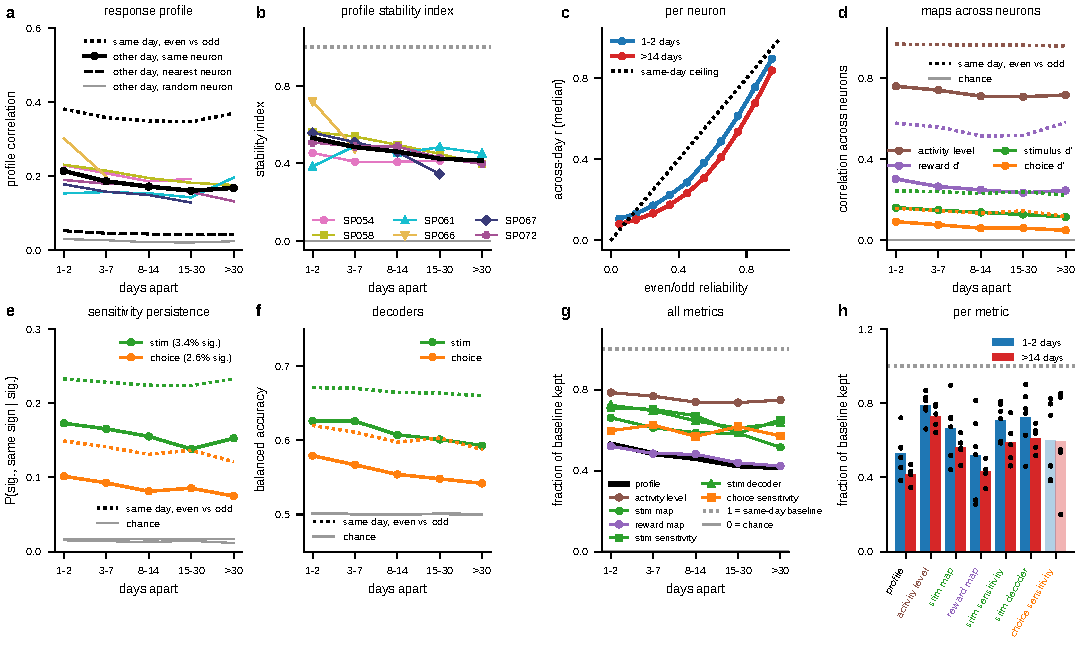
\includegraphics{chronic_stability.pdf}
\caption{\textbf{Cross-day reliability of tracked neurons, each metric against its even/odd within-session baseline.}
6 mice, 83 sessions, 644 session pairs, QC-passing matches only. Line styles throughout: dotted, same-day baseline (even vs.\ odd trials of the same session); solid with markers, across days (even trials of day $a$ vs.\ odd trials of day $b$); thin grey, chance. Colours throughout: black, response profile; brown, activity level; green, stimulus; orange, choice; purple, reward; blue and red, 1--2 and $>$14 days apart (c, h). Thin coloured lines (a) and coloured markers (b): individual mice; thick black lines: mean over mice.
\textbf{a}~Median correlation of the 27-value response profile on the same day, with the same neuron on another day, with the spatially nearest tracked neuron (dashed) and with a random neuron of the same FOV (grey, chance).
\textbf{b}~Profile stability index $(r_x-r_0)/(r_w-r_0)$ per mouse, with medians over neurons of $r_w$ (within day, w: even vs.\ odd trials of the same session), $r_x$ (across days, x: even trials of day $a$ vs.\ odd trials of day $b$) and $r_0$ (chance, 0: as $r_x$ but with a random other neuron of the same FOV).
\textbf{c}~Per neuron: median across-day correlation $r_x$ against even/odd reliability $\sqrt{r_{w,a}\,r_{w,b}}$, the geometric mean of the neuron's within-day correlations on day $a$ and day $b$; dotted: identity, the across-day value expected from the same-day noise ceiling if the profile did not change.
\textbf{d}~Population maps: for each session half, one value per tracked neuron; the map is compared by Pearson correlation across the neurons shared by the two sessions. Activity level: $\log$ of the neuron's mean deconvolved activity over all trials and windows. $d'=(\mu_1-\mu_2)/\sqrt{(\sigma_1^2+\sigma_2^2)/2}$ of single-trial activity between two trial groups: stimulus, contra- vs.\ ipsilateral stimulus in the stimulus window (0--0.3\,s); choice, the two choices in the pre-movement window ($-0.3$--0\,s); reward, rewarded vs.\ unrewarded trials in the feedback window (0--0.3\,s).
\textbf{e}~Of the neurons significantly stimulus- or choice-selective on one half ($p<0.01$), the fraction significant with the same sign on the other half; grey: chance (half the fraction of significant neurons).
\textbf{f}~Ridge decoders of stimulus side and choice; grey: chance, from decoders trained on shuffled labels.
\textbf{g}~All metrics of a, b and d--f as the fraction of their baseline kept; colour, variable; marker, metric type (circles, maps; squares, sensitivity persistence; triangles, decoders). Dotted grey at 1: as reproducible as the same-day baseline; solid grey at 0: chance. The choice map and the choice decoder are not normalised: their within-session values are close to chance, so the per-pair ratio is ill-defined.
\textbf{h}~Fraction of baseline kept at 1--2 vs.\ $>$14 days apart, per metric (label colour as in g); bars: mean over mice; dots: mice (6 at 1--2 days, 5 at $>$14 days: SP066 spans 6 days); dotted: baseline. Choice sensitivity (faded) has a baseline close to chance and is unreliable.}
\label{fig:main}
\end{figure}

\paragraph{a: Response profiles are partly preserved.}
The even/odd profile correlation within a session is modest ($\tilde r_w\approx0.36$), which sets the ceiling.
Across days the same neuron reaches $\tilde r_x=0.21$ at 1--2 days and 0.16--0.17 beyond two weeks.
This is far above the nearest tracked neuron (0.04--0.05) and a random neuron of the same FOV (0.02--0.03).
Two conclusions follow: the tracked identity carries cell-specific information that a neighbour does not share, and much of the within-day signal is not reproduced on another day.

\paragraph{b: About half of the reproducible profile survives a day, and the decline afterwards is slow.}
The stability index is 0.53\,$\pm$\,0.05 (mean\,$\pm$\,s.e.m.\ over mice) at 1--2 days and 0.42\,$\pm$\,0.02 at $>$14 days.
The trend with time is not significant across mice (slope $-0.08$ per decade of days, $p=0.09$).
Mice range from 0.38 to 0.72 at short intervals and converge to about 0.4 beyond two weeks.
Most of the loss is therefore a step between consecutive days rather than a gradual drift.

\paragraph{c: Reliable neurons keep their profile.}
Per neuron, the across-day correlation rises steeply with within-day reliability.
Neurons with even/odd reliability $>$0.9 keep $r_x\approx0.9$ at 1--2 days and $\approx$0.85 at $>$14 days, close to identity.
Unreliable neurons fall below identity.
The low population average in (a, b) therefore reflects the many weakly responsive neurons; well-driven neurons are close to fully stable.

\paragraph{d: Activity level and selectivity maps.}
These metrics ask whether the \emph{ranking} of neurons is kept, independent of each neuron's full response profile.
For each half of a session we computed one number per neuron and correlated these numbers across all neurons tracked in both sessions.
The \emph{activity level} is the log mean activity over all trials and windows: it captures which neurons are strongly or weakly active.
The \emph{selectivity maps} use $d'$, the difference of the mean single-trial responses of two trial groups divided by their pooled s.d.: contra- vs.\ ipsilateral stimulus in the stimulus window, the two choices in the pre-movement window, and rewarded vs.\ unrewarded trials in the feedback window.
Because correlation is scale-free, these maps are insensitive to session-wide changes in signal amplitude.
The activity-level map is almost perfectly reproducible within a day ($r=0.97$) and stays high across days (0.76 to 0.71): which neurons are active is largely kept.
The stimulus $d'$ map is weak even within a day ($r\approx0.25$), because few neurons are stimulus-selective, and keeps 0.16 to 0.12 across days.
The reward map is stronger within a day (0.55) but falls to 0.30 to 0.24 across days, i.e.\ reward tuning changes more than stimulus tuning relative to its baseline.
The choice map is hardly reproducible even within a session ($r\approx0.14$), so it was not normalised in g, h.

\paragraph{e: Significant selectivity persists, at reduced rate.}
Only 3.4\% (stimulus) and 2.6\% (choice) of neurons are significantly selective on half the trials.
Of the stimulus-selective neurons, 23\% are significant again with the same sign on the other half of the same session, against chance 1.7\%.
Across days this falls to 17\% at 1--2 days and 14--15\% beyond two weeks.
For choice the corresponding values are 15\% within a session and 10\% to 7.5\% across days.
The low within-session persistence shows that, at this effect size and trial count, significance on one half is a noisy label.
Relative to this ceiling, about 60--70\% of the persistence survives across days.

\paragraph{f: Population decoders transfer across days.}
A stimulus-side decoder reaches 0.67 balanced accuracy within a session.
Trained on one day, it still gives 0.63 on the next and 0.59 beyond a month.
The choice decoder drops from 0.62 to 0.58 and then 0.54. Chance, from decoders trained on shuffled labels, is 0.50 for both.
The population code for the stimulus therefore remains largely readable with a fixed decoder across weeks.

\paragraph{g, h: All metrics show the same pattern.}
Normalised by their baselines, the metrics of a, b and d--f decline in parallel (g). At 1--2 vs.\ $>$14 days (h), the fraction of baseline kept is:
activity level 0.79 vs.\ 0.73 (the only decline significant across mice, $p=0.018$);
stimulus map 0.66 vs.\ 0.56;
reward map 0.52 vs.\ 0.43;
stimulus sensitivity 0.71 vs.\ 0.59;
stimulus decoder 0.72 vs.\ 0.61.
Choice sensitivity (0.60 vs.\ 0.59) varies widely between mice because its baseline is close to chance (h). The choice decoder could not be normalised for the same reason: its within-day accuracy is often near chance, so the ratio diverges for single pairs.
The ordering is consistent: \emph{which} neurons are active is the most stable, while detailed response shapes and reward tuning are the least stable.

\begin{figure}[!t]
\centering
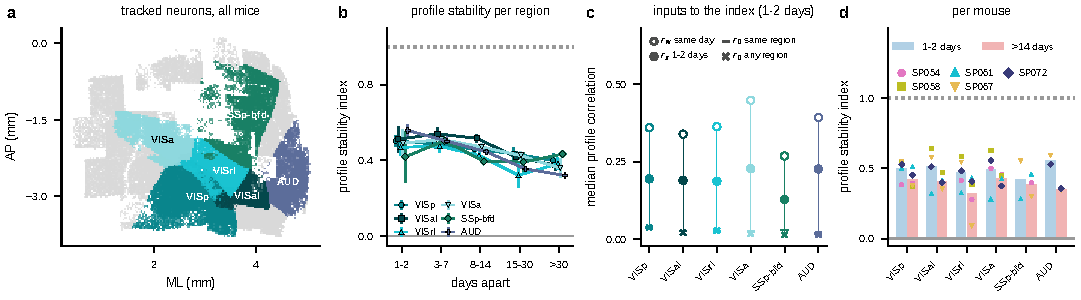
\includegraphics{regions.pdf}
\caption{\textbf{Profile stability per cortical region.} Profile stability index (Fig.~\ref{fig:main}b), computed on the tracked neurons of each region, with chance $r_0$ from a partner of the same region and FOV. Region colours are shades of the Allen atlas colours: teal for visual areas, green for SSp-bfd, and slate for AUD (whose Allen teal would clash with the visual areas). Dotted line, same-day baseline (1); grey line, chance (0); dots, mice (colours as in Fig.~\ref{fig:main}); bars, mean over mice; error bars, s.e.m.\ over mice.
\textbf{a}~Tracked neurons of all mice in a dorsal view of the CCF (ML, AP), coloured by region; other regions in grey.
\textbf{b}~Index against days apart, per region.
\textbf{c}~Inputs to the index at 1--2 days apart (medians, mean over mice). $r_w$: same day, even vs.\ odd trials (open). $r_x$: across days (filled). $r_0$: random partner of the same region (bar) or of any region (cross). The index is $(r_x-r_0)/(r_w-r_0)$.
\textbf{d}~Index at 1--2 days (blue bars) and $>$14 days apart (red bars); symbols, individual mice.}
\label{fig:regions}
\end{figure}

\paragraph{No region is clearly more stable than the others (Fig.~\ref{fig:regions}).}
Coverage differs by region (a): VISp, VISrl (5 mice), VISal and VISa (4 mice) are well sampled, SSp-bfd (3 mice) and AUD (2 mice) less so.
In all six regions the index follows the pattern of the whole population, a step at day 1 followed by a slow decline (b). It ranges from 0.42 to 0.56 at 1--2 days (VISp 0.50) and from 0.32 to 0.43 beyond 14 days (VISp 0.42).
Within-day reliability differs more between regions than stability does (c). $r_w$ is highest in VISa (0.45) and AUD (0.39) and lowest in SSp-bfd (0.27), but $r_x$ scales with it, so the fraction kept is similar.
The region-matched chance (0.02--0.04) is barely above the chance from any region. Neurons of one region therefore share little response shape beyond what all neurons share, and the index is nearly the same with either chance level (differences $\leq$0.05).
Compared within the same session pairs, no region differs consistently from VISp (not shown). Mean differences are between $-0.04$ and $+0.01$, the mice disagree in sign, and no test reaches significance (VISrl lower in 4 of 5 mice, $p=0.13$; VISal and VISa $p=1$; SSp-bfd and AUD have too few mice to test).
The decline over days is negative in nearly every mouse and region, at $-0.04$ to $-0.11$ per 10 days on average over mice (linear fit per mouse; not shown). The steeper values (VISrl, AUD) rest on single mice, e.g.\ SP067 VISrl at $-0.24$.
At the present sample size, stability of response profiles is therefore a property shared across dorsal cortex rather than one that distinguishes regions. Differences smaller than about 0.1 of the baseline cannot be excluded, and regions sampled in only 2--3 mice (SSp-bfd, AUD) need more animals.

\paragraph{Single neurons that gain or lose selectivity.}
Of 31\,577 neurons tracked in $\geq$6 QC sessions, 531 are clearly stimulus-selective.
Among these, 9.8\% lose and 7.0\% gain selectivity over days, against 2.5\% each expected by chance.
Non-selective neurons give 4.0\% and 2.7\%, close to chance.
The direction depends on the mouse: SP058 and SP072 mostly lose (13--15\%), SP067 mostly gains (16\%), and SP054 and SP061 are near chance.
This points to mouse-wide changes (training stage, imaging conditions) on top of cell-specific drift.
Example rasters are in \texttt{output/examples\_*.pdf}. They include a stable cell (SP058 9a5f5dbf, $d'\approx0.65$ over 44 days), a losing cell (b81244f9, $d'$ 0.95 $\to$ 0.2 over 35 days with an unchanged footprint), and a cell whose day-to-day swings are confirmed by agreeing even and odd trials.

\paragraph{Conclusion and caveats.}
Tracked neurons keep a clearly cell-specific response. Across days they retain about 50--80\% of what is reproducible within a session, depending on the metric.
Most of the loss occurs between consecutive days, with only a slow further decline over weeks, and well-driven neurons are close to fully stable. Profile stability is similar across the six dorsal cortical regions tested.
Caveats:
(i) The overall amplitude of the deconvolved signal varies up to $\sim$10$\times$ between sessions, so all metrics here are scale-free and absolute activity is not compared.
(ii) Only five mice contribute to the decline test.
(iii) Coverage is uneven: SP058, SP067 and SP072 end with blocks of sessions that share few neurons with earlier ones, and SP067's last two sessions share no IDs with the rest.
(iv) Regional comparisons rest on 2--5 mice per region and on the CCF registration of each FOV; neurons near region borders may be misassigned.
(v) Part of the day-1 step may come from day-specific factors (behavioural state, imaging quality) rather than changes in the neurons' tuning.

\end{document}
